\documentclass[lettersize,journal]{IEEEtran}

\usepackage{amsmath,amssymb}
\usepackage{graphicx}
\usepackage{booktabs}
\usepackage{cite}
\usepackage{balance}
\usepackage{url}
\usepackage{textcomp}
\usepackage{stfloats}
\usepackage{newtxtext,newtxmath}
\usepackage[scheme=plain,fontset=fandol]{ctex}

\title{可预测性感知软集合跳频：一种抗反应式干扰方法}
\author{作者1，作者2，作者3}

\begin{document}
\maketitle

\begin{abstract}
稀疏多载波跳频中，硬性近期集合排除将碰撞风险集中为可预测的边界尖峰。本文解析推导了这一边界暴露的闭式表达，进而提出带有包含概率上限的可预测性感知软跳频方案（PASH-cap）。在统一编码OFDM网格上，硬性记忆受限集合跳频（MCSH）在单时隙跟随干扰下误块率（BLER）为0.001，但其边界尖峰在时延三处将BLER推升至0.138；PASH-cap将其降至0.020。面对反馈辅助的因果攻击者，PASH-cap将BLER从0.123降至0.018，且在反馈损坏和延迟条件下该优势依然保持。随机跳频在概率感知攻击下仍为最优选择。综上，PASH-cap提供的是一个跨威胁折衷方案，而非普适最优解。
\end{abstract}

\begin{IEEEkeywords}
抗干扰通信，跳频，OFDM，反应式干扰，可预测性。
\end{IEEEkeywords}

\section{引言}
\IEEEPARstart{跳}{频}（FH）链路通过不断改变占用频率来规避反应式干扰，但具备历史感知能力的干扰机可利用跳频规则自身的结构规律实施攻击。该问题具有明确的现实背景：在战术通信和车联网等场景中，稀疏多载波波形必须在跟踪频谱占用的跟随式干扰下维持连通，而每次激活多个子载波的集合值跳频恰好适配这类带宽高效链路。近年来，学界提出了一系列防御方案，涵盖索引调制跳频\cite{shi2022enhanced}、数据驱动与强化学习跳频\cite{zhou2024,zhang2024block,qi2024,cheng2025,chen2026dual}、抗干扰博弈\cite{zhang2024game}以及干扰调制\cite{ma2023}等方向。检测类工作聚焦于OFDM中反应式干扰机识别\cite{altun2022reactive,wesolowski2023detection}与多节点协作感知\cite{li2024}。序列构造类工作提供了宽间隔或无碰撞区特性\cite{shu2024widegap,zheng2025widegap}，而编码OFDM研究则侧重接收端干扰缓解\cite{mailaender2013,kaplan2023,chen2023,mendonca2024channel,wu2026llr}。上述方案共享一个核心理念：无论通过组合序列约束还是学习型策略，均致力于\emph{避免}使用近期频率。

本文所追问的是一个更深层的问题：当近期频率集合被过度排除时，这种排除本身是否创造了新的脆弱性？硬性排除可保证受保护记忆窗口内的零碰撞，但同时也缩小了条件选择空间，使得紧邻记忆窗口之外的频率以不成比例的概率被重新选中。具备历史感知能力的攻击者无需观测当前活跃集合即可利用这种边界概率集中现象。值得注意的是，宽间隔和无碰撞区文献提供了在指定时延处具有可证明碰撞避免能力的确定性序列构造，然而这类构造面向的是\emph{成对}跳频模式（每符号仅一个活跃子载波），并未触及$S>1$个活跃子载波的集合值跳频中特有的条件包含集中问题。类似地，基于强化学习的策略能够通过在线碰撞反馈学会规避近期频率，却无法对自身行为所创造的暴露提供可解释的上界，其闭环特性还引入了反馈操纵的脆弱性。与优化跳频策略的思路不同，本文的核心工作是诊断记忆机制的一个结构性后果——边界尖峰——并提供一种可调的、规避在线学习收敛陷阱的开环替代方案。

本文做出三项贡献。其一，导出硬性记忆受限集合跳频（MCSH）在首个无保护滞后处碰撞的闭式表达，从解析层面揭示更深记忆为何非但不能消除边界尖峰，反而将其放大。其二，提出带有条件包含概率上限的可预测性感知软跳频方案（PASH-cap），采用固定大小系统抽样以精确实现指定的边际包含概率。其三，在统一编码OFDM网格上，于固定时延、概率感知和反馈辅助因果攻击三类威胁下系统评估Random、MCSH和PASH-cap，并通过反馈退化实验验证该暴露的结构性本质，而非完美反馈条件下的假象。

\section{系统与威胁模型}
在第$m$个OFDM符号，发射机激活子载波集合$\mathcal A_m\subseteq\{1,\ldots,N\}$，且$|\mathcal A_m|=S$。干扰机同时占据等规模集合$\mathcal J_m$，归一化碰撞定义为
\begin{equation}
 c_m=\frac{|\mathcal A_m\cap\mathcal J_m|}{S}.
\end{equation}
定义滞后$d$的自碰撞$C_d=\mathbb E[|\mathcal A_m\cap\mathcal A_{m-d}|/S]$。固定时延跟随者使用$\mathcal J_m=\mathcal A_{m-d}$，故其期望碰撞即为$C_d$。本文测试$d=1$和$d=3$两种情况。分块循环确定性构造（BCD）遍历$N/S$个正交集合，仅用作结构性压力测试：其短滞后碰撞为零，但周期性复用意味着远期模式完全可预测。

概率感知攻击者获知条件边际包含概率
\begin{equation}
p_{k,m}=\Pr(k\in\mathcal A_m\mid\mathcal A_{<m})
\end{equation}
并干扰$p_{k,m}$最大的$S$个子载波，其归一化期望碰撞等于前$S$个概率质量之和除以$S$。

反馈辅助因果攻击者为每个候选时延$d\in\{1,\ldots,6\}$维护一个指数平滑碰撞评分。每时隙前，攻击者以$\epsilon$-贪心规则选定一个时延，干扰相应的历史活跃集合；仅在动作执行后方可观测归一化碰撞值并更新该时延的评分。因此，攻击者在决策时刻无从访问当前集合$\mathcal A_m$，但其行动依赖于精确的时隙后碰撞反馈。

\begin{figure*}[!t]
\centering
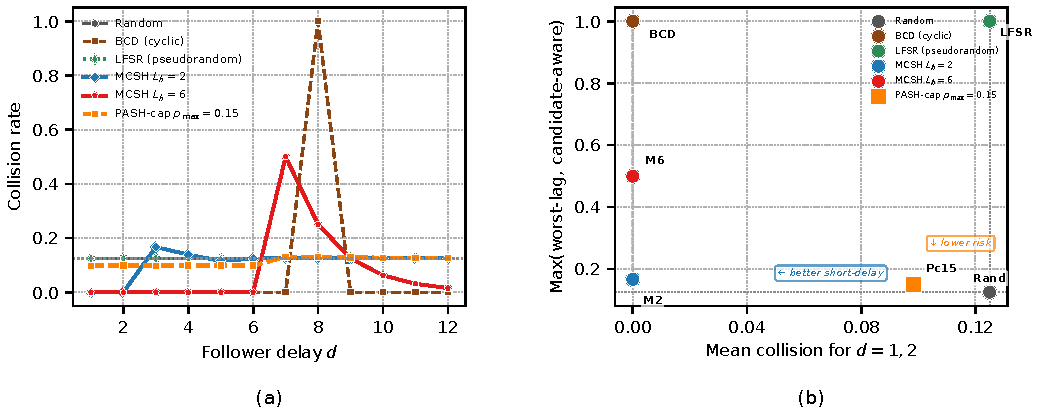
\includegraphics[width=0.96\textwidth]{../../figures/paper/comml_fig1_structural.pdf}
\caption{结构性暴露。(a) MCSH消除了受保护滞后内的碰撞，却在式\eqref{eq:boundary}处产生边界尖峰；PASH-cap限制了这种概率集中。(b) 短时延保护与最坏条件暴露之间构成根本性的折衷关系。BCD为确定性压力构造，并非外部基线方法。}
\label{fig:structural}
\end{figure*}

\section{边界暴露与PASH-Cap}
MCSH以记忆深度$L_h$在可行范围内从最近$L_h$个活跃集合的并集之外均匀选取$S$个子载波。该规则保证
\begin{equation}
\mathcal A_m\cap\mathcal A_{m-d}=\varnothing,\qquad 1\leq d\leq L_h.
\end{equation}
\textbf{命题1：}若$(L_h+1)S\leq N$，则首个无保护滞后处的碰撞为
\begin{equation}
C_{L_h+1}=\frac{S}{N-L_hS}.
\label{eq:boundary}
\end{equation}
\emph{证明：}依定义，$\mathcal A_m$与最近$L_h$个活跃集合均不相交。这$L_h$个集合至多排除$L_hS$个不同子载波，剩余$N-L_hS$个候选子载波供$\mathcal A_m$从中均匀抽取。而$\mathcal A_{m-L_h-1}$系从全部$N$个子载波中均匀抽取，其$S$个元素各以概率$(N-L_hS)/N$落入无保护补集。在该补集内，任意元素出现在独立抽取的$\mathcal A_m$中的条件概率为$S/(N-L_hS)$。乘以$S$并归一化即得式\eqref{eq:boundary}。由此可见，增大$L_h$并非消除尖峰，而是将其推迟至更远滞后并以更高幅度重现——更深的记忆非但未能解决问题，反而将其延后并放大。

\textbf{推论：}MCSH的硬性排除使无保护补集内所有子载波地位均等，条件包含概率在该补集上呈均匀分布。故概率感知暴露恰等于边界尖峰高度：$R_{\mathrm{cand}}=C_{L_h+1}=S/(N-L_hS)$。值得注意的是，无保护补集上的均匀分布已是与短滞后零碰撞约束相容的\emph{最不集中}的分布——MCSH正是在这一最温和的条件下达到了上述暴露水平；任何将概率集中于部分子载波的策略只会使$R_{\mathrm{cand}}$更高。零短滞后碰撞因此并非无代价：它伴随着随$L_h$增长而不可避免的可预测性代价。

PASH-cap以基于近期使用次数的指数衰减惩罚替代硬性排除。在候选衰减函数中，指数形式兼具三个实用优点：权重对所有有限计数保持严格正值（避免了复制MCSH边界问题的硬置零），仅需单一参数$\alpha$控制整体衰减速率，且当$\alpha\geq1.4$时超过$H$步的历史贡献自然趋于可忽略，免除了显式截断的必要。该形式在无需引入脆性阈值的前提下，刻画了重复频率规避的边际可预测性增益递减规律。给定记忆深度$H$，定义子载波权重
\begin{equation}
w_{k,m}=p_{\mathrm{floor}}+
\exp\!\left[-\alpha\sum_{\ell=1}^{H}\mathbf 1\{k\in\mathcal A_{m-\ell}\}\right].
\end{equation}
目标边际概率通过带上限的归一化求得，
\begin{equation}
p_{k,m}=\min\{p_{\max},\eta_m w_{k,m}\},\qquad \sum_{k=1}^{N}p_{k,m}=S,
\label{eq:cap}
\end{equation}
其中缩放因子$\eta_m$由二分法确定。为精确实现这些边际概率，PASH-cap采用固定大小系统抽样：先将$N$个子载波随机排列，抽取均匀偏移量$u\sim\mathcal U[0,1)$，采样器依次检查累积和$\{p_{k,m}\}$（按排列顺序），选中所有包含任一阈值$u,u+1,\ldots,u+S-1$的区间所对应的子载波。因$\sum_k p_{k,m}=S$，$S$个阈值各跨越一个单位的累积质量，且$p_{k,m}\leq p_{\max}\leq1$保证单个子载波至多被一个阈值穿过，故恰好选出$S$个不同子载波。随机排列下的可交换性确保子载波$k$的包含概率恰好为$p_{k,m}$。

对于任意有效边际概率，概率感知暴露
\begin{equation}
R_{\mathrm{cand}}=\frac{1}{S}\sum_{k\in\operatorname{TopS}(\boldsymbol p_m)}
p_{k,m}
\end{equation}
满足$S/N\leq R_{\mathrm{cand}}\leq p_{\max}$。随机跳频触及下界，PASH-cap则通过$p_{\max}$显式上限控制了为近期频率规避所付出的可预测性代价。本文取$H=6$、$\alpha=1.4$、$p_{\mathrm{floor}}=0.20$、$p_{\max}=0.15$。计算近期使用计数、上限归一化和系统抽样的总开销为$O(NH)$（直接实现）加$O(N+S)$（抽样）。不同于MCSH——命题1为其边界尖峰给出了精确闭式表达——PASH-cap下的$C_d$并无同类简易解析式：软权重引入的序列相关性抵制初等分析，因此第IV节报告的编码实验结果构成PASH-cap性能的主要量化依据。

上述参数通过结构化扫描确定，扫描范围覆盖$\alpha\in[0.4,2.0]$、$p_{\mathrm{floor}}\in[0.10,0.35]$、$p_{\max}\in[0.12,0.20]$，以$\max(R_{\mathrm{hist}},R_{\mathrm{cand}})$最小化为目标，约束$R_{\mathrm{short}}\leq0.10$且子载波利用率变异系数$\geq0.025$（共180个网格点）。结构最优解为$(\alpha{=}1.4,p_{\mathrm{floor}}{=}0.20,p_{\max}{=}0.14)$，对应的$R_{\mathrm{short}}{=}0.104$，$R_{\mathrm{risk}}{=}0.139$。将$p_{\max}$从$0.15$收紧至$0.14$使最坏情况暴露降低$7\%$，代价是短时延碰撞增加$6\%$。编码实验表明两种上限设置在大多数威胁条件下BLER无显著差异；本文报告$p_{\max}{=}0.15$，因其为短时延保护提供了更保守的取值。

从系统设计角度看，PASH-cap与MCSH及Random共享一个关键属性：三者均为开环规则，跳频模式的生成不依赖于对干扰机行为的观测。这与基于强化学习的跳频策略形成鲜明对比——后者需要在线碰撞反馈和持续策略更新。开环特性意味着PASH-cap不存在学习延迟，不对反馈可用性做任何假设，且从根本上免疫于攻击者伪造反馈报告的风险——而这正是任何闭环防御难以根除的威胁。其代价则由概率感知攻击下的结果揭示：开环规则无法利用仅通过反馈才能获知的攻击者盲区。

一个简单的在线学习基线实验直观地印证了上述风险。我们在与因果攻击者相同的每符号精确碰撞反馈条件下，实现了基于EMA碰撞评分的$\epsilon$-贪心子载波选择器（$\epsilon{=}0.10$，$\alpha{=}0.10$）。在12~dB下面对全部四种威胁时，其BLER超过0.99——利用机制收敛至准静态子载波集合，干扰机得以完美跟踪。即使将探索率提至$\epsilon{=}0.50$或将学习率提至$\alpha{=}0.50$，BLER仍处于0.50--0.99区间，远差于随机跳频。这一负面结果表明：缺乏显式可预测性控制的在线学习可能比完全不学\emph{更为糟糕}——学习过程收敛所形成的规律性，恰恰成为干扰机攻击的靶标。

\section{实验结果}
\subsection{实验设置}
所有方法共用一套物理层参数：$N=512$子载波，$S=64$活跃子载波，QPSK调制，码率$1/2$的截断K7卷积码，混合似然软输入维特比接收机，AWGN信道（$E_s/N_0{=}12$~dB），干信比5~dB。每帧含32个OFDM符号。结构统计基于30个独立种子、5000符号长度的跳频序列。编码实验至少运行2000帧，当累积帧错误数达到100或总帧数达到5000时停止。报告百分位自助法95\%置信区间作为描述性不确定性度量。所有正式运行记录完整的配置参数、源码及输出哈希值和停止条件。七项自动验证检查确保：因果动作未接收当前活跃集、全部因果动作来自可用历史集、固定种子下攻击轨迹可精确复现、接收机评估顺序不影响攻击轨迹、延迟反馈未被提前使用、抽样量固定及边际概率精确保持。

\subsection{结构机理}
图\ref{fig:structural}(a)从实验角度验证了式\eqref{eq:boundary}。随机跳频在所有滞后处稳定在$S/N=0.125$附近。MCSH取$L_h=2$时$C_1=C_2=0$、$C_3=64/(512-128)=1/6\approx0.167$；取$L_h=6$时$C_7=64/(512-384)=1/2=0.500$。中间记忆深度的数据确认了单调趋势：$L_h=1$给出$C_2\approx0.143$，$L_h=4$给出$C_5\approx0.250$。尖峰高度按$S/(N-L_hS)$单调增长——更深记忆并未消除暴露，只是将其推至更远滞后并以更强幅度集中体现。PASH-cap接受非零短时延碰撞（$C_1\approx0.098$），但最坏历史碰撞（$0.130$，出现在$d{=}7$）和概率感知暴露（$0.150$）均保持在随机基线附近。图\ref{fig:structural}(b)展示了由此产生的保护--可预测性折衷关系：MCSH家族沿对角线排列，较低的短时延暴露必然对应较高的最坏风险；而PASH-cap占据了硬性排除规则无法到达的区域。

\begin{figure*}[!t]
\centering
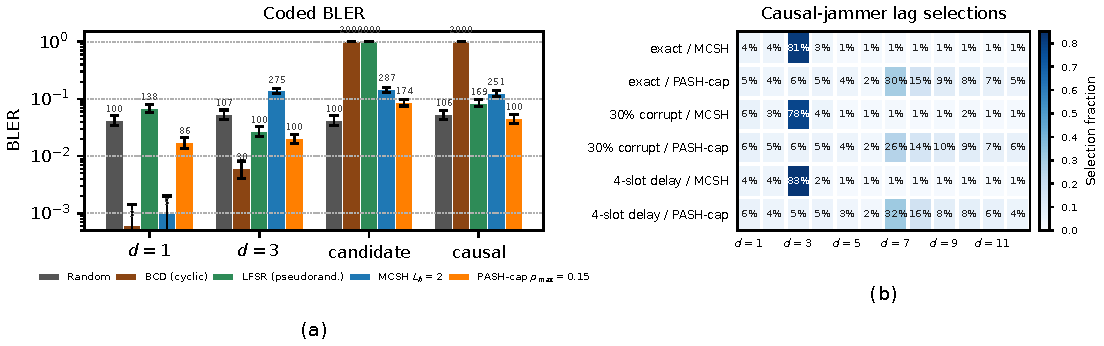
\includegraphics[width=0.96\textwidth]{../../figures/paper/comml_fig2_compact.pdf}
\caption{编码与反馈鲁棒性结果。(a) 误块率及自助法95\%置信区间，柱上数字为观测帧错误数。(b) 因果干扰机在精确反馈、报告损坏和反馈延迟条件下的滞后选择分布，各行独立归一化。}
\label{fig:compact}
\end{figure*}

\subsection{编码可靠性}
图\ref{fig:compact}(a)和表\ref{tab:bler}共同表明：没有哪一种跳频规则能在所有攻击下全面占优。面对已知的单时隙跟随者，MCSH-L2凭借硬性排除几乎将碰撞降为零，取得0.0010的BLER，PASH-cap和Random分别为0.0172和0.0425。然而在$d{=}3$处——恰在MCSH-L2的记忆保护边界之外——边界尖峰将BLER推升至0.1375，相较$d{=}1$恶化了约138倍。PASH-cap因无边界集中现象而保持在0.0200，同时优于MCSH-L2和Random（0.0535）。反馈辅助因果攻击者学到了同一$d{=}3$暴露：针对MCSH-L2，其将$>80\%$的捕获后动作集中于$d{=}3$（图\ref{fig:compact}(b)），造成0.1230的BLER；面对PASH-cap则无法形成主导滞后，仅达0.0183，本质上与固定$d{=}3$的结果一致。

MCSH-L2与PASH-cap在$d{=}3$处的BLER差距（0.1375对0.0200，相差6.9倍）远大于二者的平均碰撞率差距（0.167对0.100，仅差1.67倍）。这一非线性现象根源于边界尖峰与信道编码之间的交互机制。MCSH-L2在$d{=}3$下，干扰机恰将三个符号前的模式移位复现，在帧内形成时间簇集的连续碰撞，直接压垮卷积码的纠错裕度。PASH-cap的软概率控制则使碰撞均匀散布于各符号与各帧之间，码率$1/2$的卷积码得以从低强度、均匀分布的碰撞中恢复。由此可见，碰撞到BLER的映射不由平均碰撞率决定，而由帧内碰撞的\emph{集中程度}决定——这正是边界尖峰所致危害的核心。

在完全概率感知条件下，随机跳频达到理论下界（BLER 0.0422），因其均匀的$p_{k,m}$未向攻击者提供可利用的概率集中。PASH-cap因$p_{k,m}$非均匀但受上限约束，BLER为0.0870——虽不及随机跳频，但显著优于BLER达0.1435的MCSH-L2，后者的硬性排除创造了高度集中的条件概率分布。

在$E_s/N_0{=}9$~dB下重复相同实验，确认方法排序在更低信噪比下依然保持，PASH-cap在$d{=}3$处相较MCSH-L2的改善倍数为6.3。当干信比升至10~dB（SNR固定于12~dB），排序再次保持一致，且PASH-cap的优势进一步扩大：$d{=}3$处改善倍数达9.4（0.1760对0.0188），面对因果攻击者达7.9（0.1525对0.0194）。变SNR和变JSR实验一致表明，随机跳频在概率感知攻击下始终是最强选择。完整敏感性实验数据以补充材料形式提供。

\subsection{反馈鲁棒性}
图\ref{fig:compact}(b)检验了因果攻击的实验优势是否依赖于完美反馈假设。本文考察两种退化场景：以0.30的概率将真实碰撞报告替换为无信息基线$S/N$，或为反馈施加四个额外时隙的延迟。在所有三种条件下（精确反馈、30\%损坏、4时隙延迟），MCSH-L2均将80.0\%--83.6\%的捕获后动作分配给$d{=}3$，碰撞率0.146--0.147，BLER 0.114--0.124。边界尖峰之显著以至于即使反馈严重退化，攻击者仍不偏移——这说明暴露是结构性的，并非精确即时反馈条件下的假象。PASH-cap在所有条件下保持滞后选择的高度分散，碰撞率稳定在0.097，BLER保持在0.0157--0.0183。软概率上限从根本上阻止了碰撞在任何单一滞后处集中，从而无论反馈质量如何，攻击者均无从获取可学习的集中模式。反馈鲁棒性实验中PASH-cap的数据点为每条件3000帧中46--63帧错误，其置信区间虽宽于表\ref{tab:bler}的区间，但在所有条件下均与MCSH-L2的区间完全分离。

\begin{table}[!t]
\centering
\caption{误块率（BLER）及自助法95\%置信区间}
\label{tab:bler}
\scriptsize
\setlength{\tabcolsep}{2.0pt}
\begin{tabular}{lccc}
\toprule
攻击类型 & Random & MCSH-L2 & PASH-cap \\
\midrule
$d=1$ & .0425 [.035,.051] & \textbf{.0010} [.000,.002] & .0172 [.014,.021] \\
$d=3$ & .0535 [.044,.064] & .1375 [.123,.153] & \textbf{.0200} [.016,.024] \\
概率感知 & \textbf{.0422} [.035,.051] & .1435 [.129,.159] & .0870 [.075,.099] \\
因果攻击 & .0476 [.039,.057] & .1230 [.109,.138] & \textbf{.0183} [.015,.022] \\
\bottomrule
\end{tabular}

\vspace{3pt}
{\scriptsize 粗体为每行三种方法中最佳值。百分位自助法95\%置信区间（混合似然软输入维特比接收机）。PASH-cap各点均达到100帧错误统计目标（$d{=}1$: 86/5000; $d{=}3$: 100/4999; 因果: 100/5457（延长运行）; 概率感知: 174/2000）。}
\end{table}

\subsection{适用范围与设计启示}
本文所有实验基于AWGN信道假设；9~dB SNR和10~dB JSR的敏感性测试确认方法排序保持不变。在频率选择性衰落环境中，碰撞的危害程度将与子载波的信道质量相关——这一交互效应留待后续工作探索。本文的比较工作在一个编码AWGN链路上独立考察了跳频模式暴露的影响，并不声称优于已发表的RL、无碰撞区或OFDM-IM等方法。概率感知攻击者假设获知精确的条件边际概率，因果攻击者则假设获得时隙后碰撞反馈。这两种信息模型是经过权衡选择的上界情形，旨在界定设计空间的两极，而非穷举刻画实际对手。自适应停止规则和单条连续因果轨迹的实验设定也意味着，报告的自助法区间应理解为描述性不确定性度量。

尽管存在上述边界，实验结果仍为工程实践提供了一条清晰的决策逻辑。当跟随者时延已知且较短时，匹配记忆深度的MCSH是确定性的最优选择。当时延不确定或攻击者具备在线自适应能力时，PASH-cap既能避免硬性排除在记忆失配时的灾难性边界尖峰退化，又能保留有效的短时延保护。而当攻击者的信息能力接近完全掌握跳频分布时，构造上即最小化条件概率暴露的随机跳频反而最优。PASH-cap恰好填补了两种极端之间的空白地带：通过单一参数$p_{\max}$直接约束最坏情况条件暴露，使得保护--可预测性折衷变得既可解释又可调节。

\balance
\section{结论}
本文识别并量化了稀疏多载波跳频中硬性近期集合排除的一个结构性失效模式：受保护记忆窗口内的零碰撞保证，以可预测的边界尖峰为代价——尖峰幅度按$C_{L_h+1}=S/(N-L_hS)$随记忆深度增大而单调上升。历史感知型或自适应攻击者无需获知当前活跃集合，即可学习并锁定这一尖峰，反馈辅助因果攻击者的行为已充分验证了这一点。

PASH-cap以指数衰减的软惩罚和显式逐子载波概率上限取代硬性排除。它虽牺牲了MCSH在已知短时延下的最优性，且在完全概率感知下不能超越随机跳频，但在$d{=}3$处相较MCSH将编码BLER改善了6.9倍，面对因果攻击者改善6.7倍，并在退化反馈条件下保持上述增益。上限参数$p_{\max}$直接约束了最坏情况条件暴露，使保护--可预测性折衷变得既可解释又可调节。后续工作应评估衰落信道下的性能、依赖信道感知的反馈模型，并在硬件平台上验证这一折衷方案。

\section*{数据可用性}
程序代码和配置文件可向作者索取。9~dB SNR和10~dB JSR的敏感性实验数据以补充材料形式提供。

\bibliographystyle{IEEEtran}
\bibliography{../references_ieee}

\end{document}
